\section{685 --- Redundant Connection II}
In this problem, a rooted tree is a \textbf{directed} graph such that, there is exactly one node (the root) for which all other nodes are descendants of this node, plus every node has exactly one parent, except for the root node which has no parents.

The given input is a directed graph that started as a rooted tree with $ N $ nodes (with distinct values $ 1, 2, \ldots, N $), with one additional directed edge added. The added edge has two different vertices chosen from 1 to $ N $, and was not an edge that already existed.

The resulting graph is given as a 2D-array of edges. Each element of edges is a pair $ [u, v] $ that represents a directed edge connecting nodes $ u $ and $ v $, where $ u $ is a parent of child $ v $.

Return an edge that can be removed so that the resulting graph is a rooted tree of $ N $ nodes. If there are multiple answers, return the answer that occurs last in the given 2D-array.

\paragraph{Example 1:}

\begin{flushleft}
Input: \lstinline[language=C++, basicstyle=\small\ttfamily, keywordstyle=\bfseries\color{green!40!black}]|[[1,2], [1,3], [2,3]]|

Output: \lstinline[language=C++, basicstyle=\small\ttfamily, keywordstyle=\bfseries\color{green!40!black}]|[2,3]|

Explanation: The given directed graph will be like this:

\begin{figure}[H]
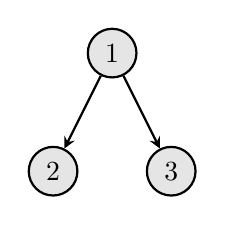
\begin{tikzpicture}
[every node/.style={draw, circle, fill=gray!20!, minimum size=5mm},
thick, >=stealth, ->]
\node{1}
child{node{2}}
child{node{3}};
\end{tikzpicture}
\end{figure}

\end{flushleft}

%  1
% / \
%v   v
%2-->3

\paragraph{Example 2:}
\begin{flushleft}


\textbf{Input}: \lstinline[language=C++, basicstyle=\small\ttfamily, keywordstyle=\bfseries\color{green!40!black}]|[[1,2], [2,3], [3,4], [4,1], [1,5]]|

\textbf{Output}: \lstinline[language=C++, basicstyle=\small\ttfamily, keywordstyle=\bfseries\color{green!40!black}]|[4,1]|

\textbf{Explanation}: The given directed graph will be like this:
\begin{figure}[H]
\begin{tikzpicture}
[every node/.style={draw, circle, fill=gray!20!, minimum size=5mm},
>=stealth, ->, thick]
\node(5){5};
\node[right=8mm of 5](1){1};
\node[right=8mm of 1](2){2};
\node[below=8mm of 1](4){4};
\node[below=8mm of 2](3){3};
\draw (1) -- (5);
\draw (1) -- (2);
\draw (4) -- (1);
\draw (2) -- (3);
\draw (3) -- (4);
\end{tikzpicture}
\end{figure}
\end{flushleft}
%5 <- 1 -> 2
%     ^    |
%     |    v
%     4 <- 3
\paragraph{Note:}

\begin{itemize}
\item The size of the input 2D-array will be between 3 and 1000.
\item Every integer represented in the 2D-array will be between 1 and $ N $, where $ N $ is the size of the input array.
\end{itemize}

\subsection{Union Find}
There are three cases in which a redundant edge exists.

\begin{enumerate}
\item No loop but there is a node with in-degree equal to 2. For example, 3 is the node in the following picture
\begin{figure}[H]
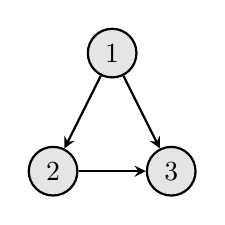
\begin{tikzpicture}
[every node/.style={draw, circle, fill=gray!20!, minimum size=5mm},
>=stealth, ->,thick]
\node{1}
child{node(2){2}}
child{node(3){3}};
\draw (2) -- (3);
\end{tikzpicture}
\end{figure}
\item A loop exists. All nodes have in-degree 1 or 0. as following example

\begin{figure}[H]
\begin{tikzpicture}
[every node/.style={draw, circle, fill=gray!20!, minimum size=5mm},
>=stealth, ->, thick]
\node(5){5};
\node[right=8mm of 5](1){1};
\node[right=8mm of 1](2){2};
\node[below=8mm of 1](4){4};
\node[below=8mm of 2](3){3};
\draw (1) -- (5);
\draw (1) -- (2);
\draw (4) -- (1);
\draw (2) -- (3);
\draw (3) -- (4);
\end{tikzpicture}
\end{figure}

\item A loop exists and one node has one in-degree 2. An example is shown as below

\begin{figure}[H]
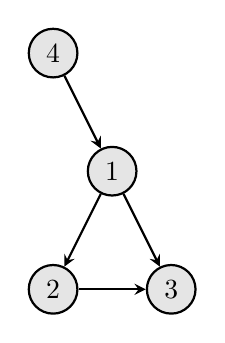
\begin{tikzpicture}
[every node/.style={draw, circle, fill=gray!20!, minimum size=5mm},
>=stealth, ->, thick]
\node{4}
child[missing]
child{node{1} child{node(2){2}} child{node(3){3}}};
\draw (2) -- (3);
\end{tikzpicture}
\end{figure}

\end{enumerate}

We process these 3 cases differently. 

\begin{itemize}
\item For the first case, we return the edge that has the node with in-degree 2 (i.e, $(2,3)$ in the example). 

\item To the 2nd case, we return the edge that form the loop (i.e., $(4,1)$ in the example.)

\item In the 3rd case, we return the edge that form the loop and contains the node with in-degree 2 (i.e., $(3,1)$ in the example).
\end{itemize}


We make use of an array $P$. For an edge $(u,v)$, this is $u\to v$, so $P[v]=u$. Initially all elements in $P$ are set to $-1$.

We start by looking for the node with in-degree equal to 2. Iterate the given edges array, for current edge $(u, v)$, if $P[v] \geq 0$, node $v$ will be the node with in-degree equal to 2. We save both previous edge $(P[v], v)$ and current edge $(u,v)$ as $e_1$ and $e_2$.

Next, we searching for loop using union find by traversing input edges again. Whenever we find a loop, we will check if $e_0$ exists or not. If $e_0$ does exist, we just return $e_0$ (case 3). Otherwise, we return current edge which forms a loop (case 2).

Finally, if we don't return during the traversing, we will return $e_2$ (case 1).

\setcounter{lstlisting}{0}
\begin{lstlisting}[style=customc, caption={Union Find}]
vector<int> findRedundantDirectedConnection( vector<vector<int>>& edges )
{
    int N = static_cast<int>( edges.size() );

    vector<int> parents( N + 1, 0 );

    vector<int> e1;
    vector<int> e2;

    //check node with in-degree 2
    for( auto& edge : edges )
    {
        int src = edge[0];
        int dst = edge[1];

        if( parents[dst] == 0 )
        {
            parents[dst] = src;
        }
        else
        {
            //dst has in-degree 2
            //save previous edge and current edge
            e1.assign( {parents[dst], dst} );

            e2 = edge;

            //invalidate edge
            edge[1] = -1;
        }
    }

    //check for loop
    for( int i = 1; i <= N; ++i )
    {
        parents[i] = i;
    }

    for( const auto& edge : edges )
    {
        if( edge[1] < 0 )
        {
            continue;
        }

        int p0 = find( parents, edge[0] );
        int p1 = find( parents, edge[1] );

        if( p0 == p1 )
        {
            //loop
            if( e1.empty() )
            {
                return edge; //case 2
            }
            else
            {
                return e1; //case 3
            }
        }

        //link edge[0] and edge[1]
        parents[p1] = p0;
    }

    //case 1
    return e2;
}

int find( vector<int>& parents, int x )
{
    while( parents[x] != x )
    {
        x = parents[x];
    }

    return x;
}
\end{lstlisting}


